%!TEX root = ../dissertation.tex

\chapter{Solution}
\label{chapter:solution}


\section{Overview}
We set out to create an \gls{ide} for \gls{gd} programming that is available from a web page.

There are five related tasks that the environment needs to support in order to be useful for the architect:
(1) it needs to let the architect develop programs;
(2) it needs to run programs;
(3) it needs to display their results;
(4) it needs to make it easy to understand programs;
and (5) it needs to export results to \gls{cad} applications.

To accomplish these tasks, there are two separate components, as seen in Figure~\ref{fig:archi:sol}: (1) the web page, where the \gls{ui} for creating programs is; and (2) the remote CAD service, that offers an \gls{api} for running programs in \gls{cad} applications.
The first four tasks can be handled by the web page alone since there is no need to interact with \gls{cad} applications running in the user's computer.
The fifth task requires both the web page and the remote CAD service.
As also seen in Figure~\ref{fig:archi:sol}, apart from using the web page programming environment \gls{ui}, the architect also needs to install the remote CAD application when he wants to export results to \gls{cad} applications.

In the rest of the chapter, we describe these two components and how each of the tasks is implemented.

We start by looking at the web page.

\begin{figure}
  \centering
  
\includegraphics[width=0.8\textwidth]{./images/architecture_overview/architecture_overview}
  \caption{Architecture of the solution.}
  \label{fig:archi:sol}
\end{figure}


\section{Web page}
To handle the tasks of letting the architect develop programs, running programs, supporting program understanding, and displaying results, the web page has the layout shown in Figure~\ref{fig:page:view}.
Taking up most of the screen space are a text editor and a 3D view that allow the architect to edit a program and view its results.
On top of the text editor and the 3D view are controls for the running process, including whether to run automatically and whether to collect data to display traceability.
To the left are hidden panels for actions like selecting a program and exporting to \gls{cad} applications.
{\bf(pictures of panels)}

To help with the implementation, we have used the THREE.js library\footnote{\url{https://threejs.org/} (last accessed on 10/10/2016)}, to interact with WebGL\cite{marrin2011webgl}, and the Ace Editor library\footnote{\url{https://ace.c9.io} (last accessed on 10/10/2016)}, to provide a syntax highlighted text editor.
{\bf(React, escodegen, esprima, estraverse, redux)}

%{\bf(describe high-level view of the inner workings of the page)}

\begin{figure}
  \centering
  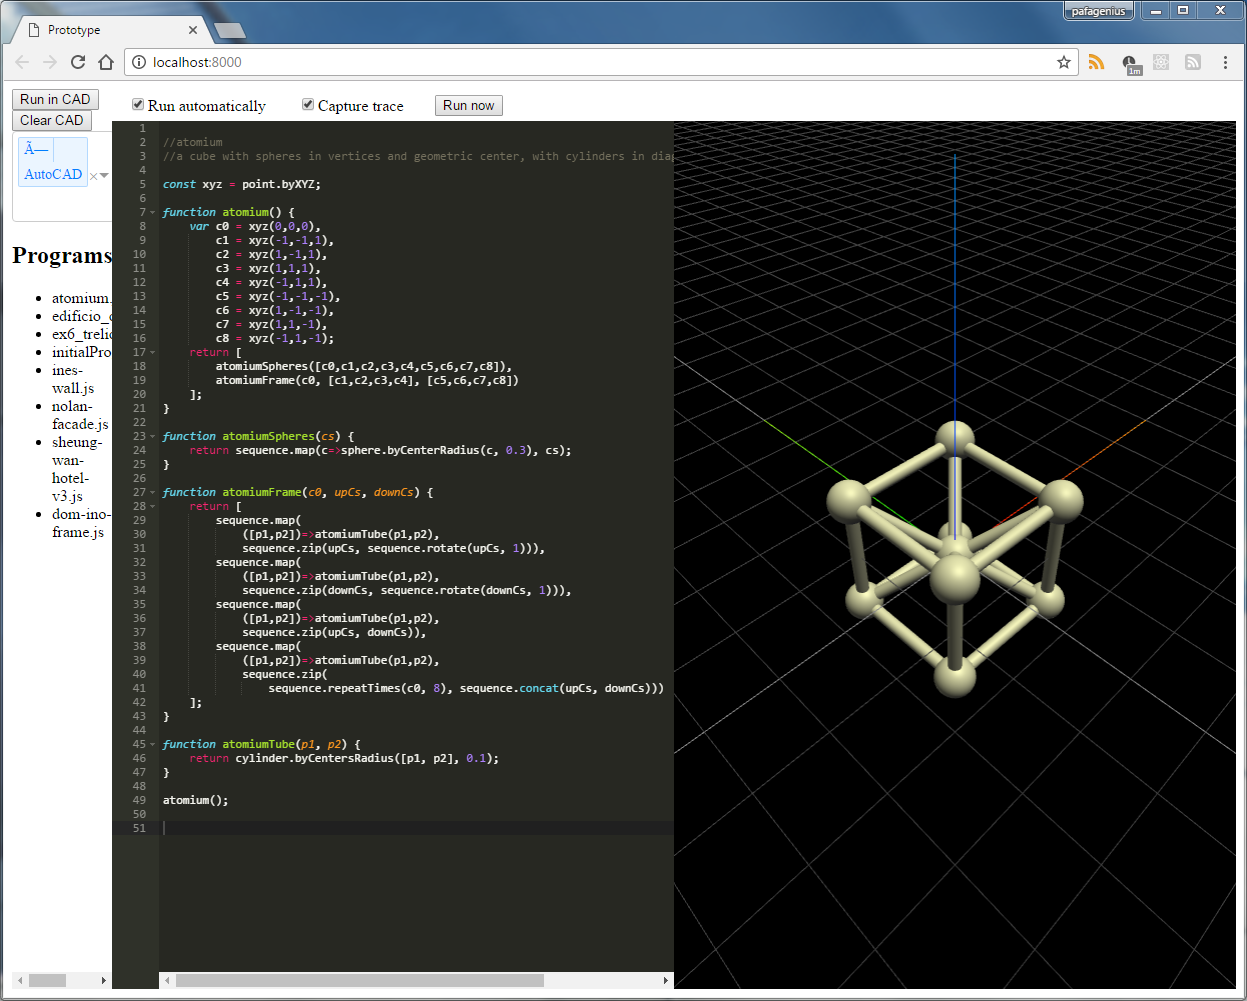
\includegraphics[width=12cm]{./images/webpage_view}
  \caption{An example view of the web page.}
  \label{fig:page:view}
\end{figure}


\subsection{Understanding Programs}
In \gls{gd}, the architect interacts with the program that creates the model instead of creating it directly in a \gls{cad} application.
This allows him to automate tasks that normally take too much time and, therefore, also allows him to explore a design space with much more repetition.
However, since he is not directly interacting with the model, he needs to understand the relationship between program and results in order to know how to change the program to get the model he wants.
Our environment enables him to do this by providing immediate feedback to changes and by showing traceability.


\subsubsection{Immediate Feedback}
\label{sec:immediate:feedback}
One of the ways to understand the program is to understand the relationship between its inputs and outputs, that is, understanding how each input affects the output model.
To do this, the architect needs to change the inputs, run the program, see the output, and repeat until he understands the relationship.
This is a tedious process that will bore must architects.
The environment can help by making this process more immediate.
It must provide quick ways of changing inputs and it must rerun the program when inputs change so the architect can see the effects of his changes immediately.
This immediacy lets the architect understand the relationship quickly which means he can start to explore the design sooner.

\paragraph{Adjusting literals}
When a value, such as a number, is typed directly into a program's source code, it is called a literal value, or simply a literal.
When experimenting with a \gls{gd} program, architects find themselves repeatedly adjusting literals that were hardcoded into the program.
This is usually done by retyping parts of the literal's text and then re-running the program to see the effect.
Unfortunately, this is annoying and, worse, it makes it difficult to fine-tune the literal.
One possible way to improving this behavior is to automatically re-run the program on every change.
This has the advantage of allowing immediate feedback to changes in literals.

However, editing literals this way often leads to errors, since it is easy to mistype characters.
The architect can increase the literal's value by an order of magnitude if, by mistake, he inserts one character without removing another.
Furthermore, when increasing the literal in steps, different hand movements are required when the increment results in a carry over, yet again increasing both the likelihood of mistyping and the time it takes to make the changes.
These errors get amplified when the programming environment provides real time feedback and, like so, begins rerunning the program before the error is corrected, leading to annoyance and to reduced \gls{ui} responsiveness.

To make this interaction more user friendly and less prone to errors, we decided to simplify the task.
Instead of retyping the literal, it would be easier to perform a simpler task, like moving the mouse or pressing a specific key on the keyboard.

\paragraph{Alternative ways of adjusting literals}
There are several ways we can extend the user interface to make adjusting literals more user friendly that do not involve manually replacing digits.
They have a simpler mapping to the user's intent.
The following list describes some of them:

\begin{itemize}
  \item {\bf Virtual joystick} Clicking on a literal will display a virtual joystick close to it. When clicked and dragged, it changes the value repeatedly over time, being faster or slower depending on how much the handle is moved from its center.
  \item {\bf Click and drag} Clicking and dragging on a literal will change it according to how much the pointer moved from the starting position.
  \item {\bf Sliders} Clicking on a literal will display a slider. Dragging the slider's handle will change the literal depending on how much the handle is moved from the center of the slider. The slider can have different scales, linear or non-linear, to map the center-handle distance to the amount of change for the literal.
  \item {\bf Keyboard shortcuts} Pressing key combinations while having a literal selected, or the text editor's caret on it, will increment or decrement the literal.
\end{itemize}

Each of the above has its advantages and disadvantages.
The {\it Virtual joystick} and the {\it Sliders}, for example, have the advantage that they are visible to the user and, like so, are easier for him to see and understand.
However, by being visible, they can also block parts of the program that he may want to see.
The {\it Keyboard shortcuts} have the advantage that they do not introduce any visual clutter into the program editor, are more precise, and that they are accessible without getting the hands out of the keyboard.
However, they do require the user to learn their key combinations, which is often avoided by new users.
Lastly, the {\it Click and drag} also has the advantage of not introducing visual clutter into the editor.
Moreover, as with {\it Virtual joystick} and {\it Sliders}, since the interaction is made using the mouse, it is more intuitive for new users.
However, less visual clutter means that the user may not realize that it is possible to adjust the literal.

Taking the advantages and disadvantages of each alternative into account, we decided to implement the {\it Click and drag} way of adjusting literals since it is a good comprise between being easy to use for new users and introducing visual clutter to the editor.
%Instead of retyping the literal, the user can just ``Click and drag'' on the literal to change its value.
Figure~\ref{fig:lit:adjust} shows an example of its usage.

\paragraph{Implementation}
To implement this behavior, we need to focus on the program editor, as this is where the relevant information is.

The behavior starts when the user presses a mouse button while the pointer is over the text editor.
If it is indeed hovering a numerical literal, we setup an event listener that will update the literal every time the pointer moves until the mouse button is released.

To check that the pointer is over a numerical node, we use the pointer position and the \gls{ast} of the current program.
Since the program will change during the behavior, we keep the path taken through the \gls{ast} to the numerical literal.
We also keep the starting pointer position as a reference for calculating the new literal value when the mouse is moved.

We update the literal by changing the portion of the source code that it represents to the digits representing the new value.
The new value has the same number of fractional digits as the original literal.
To get the new value, we first extract the number of fractional digits and an integer containing the literal's digits and sign (ignoring the decimal point) from the literal's source text.
Afterwards, we add the horizontal distance between the starting point and the current pointer position to the number.
Finally, we convert it back to text and re-add the decimal point.

\begin{figure}
  \centering
  \begin{subfigure}[b]{0.3\linewidth}
    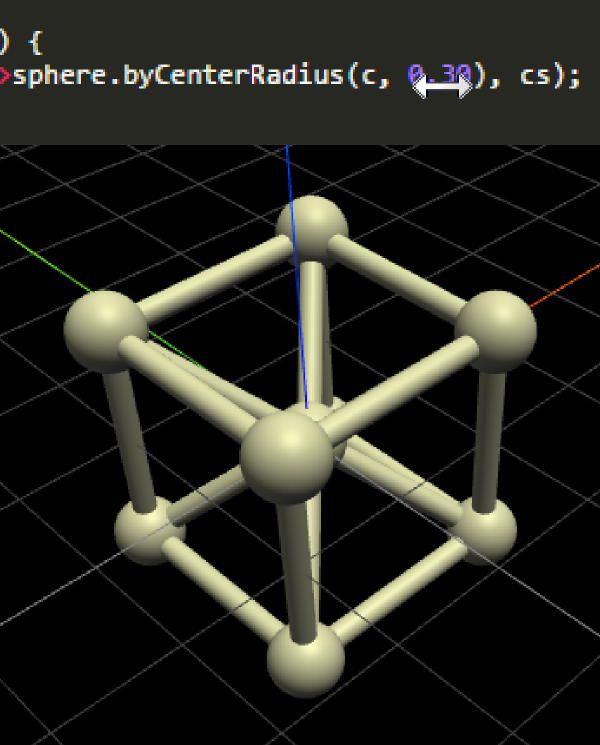
\includegraphics[width=1.0\linewidth]{./images/literal_adjustment/start_crop}
    \caption{Right after clicking.}
  \end{subfigure}
  \begin{subfigure}[b]{0.3\linewidth}
    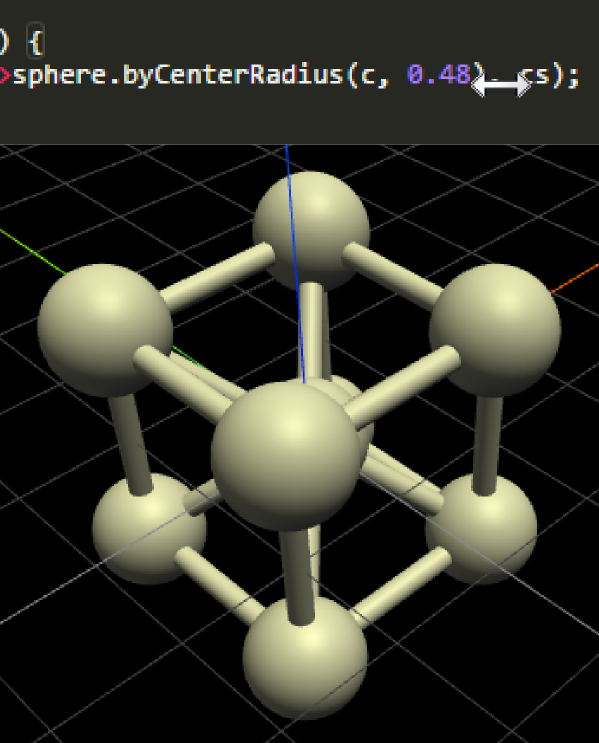
\includegraphics[width=1.0\linewidth]{./images/literal_adjustment/middle_crop}
    \caption{After dragging a little.}
  \end{subfigure}
  \begin{subfigure}[b]{0.3\linewidth}
    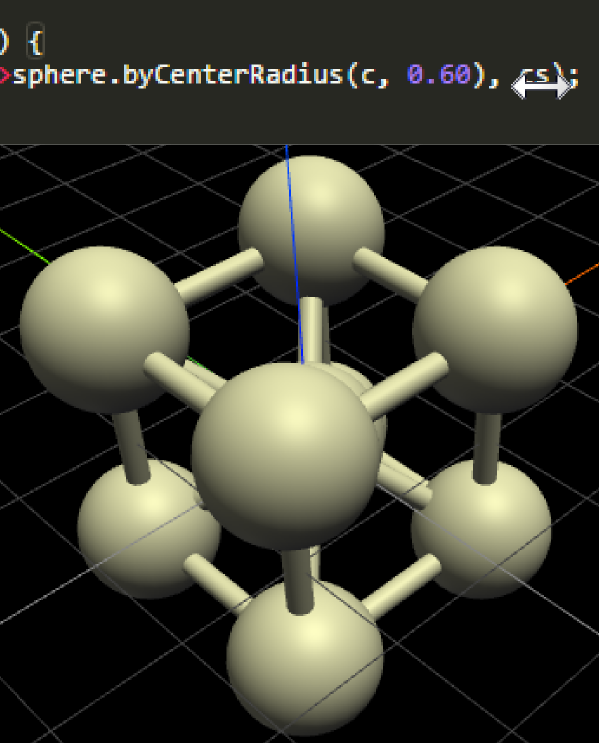
\includegraphics[width=1.0\linewidth]{./images/literal_adjustment/end_crop}
    \caption{After dragging a little more.}
  \end{subfigure}
  \caption{Example of literal adjustment.}
  \label{fig:lit:adjust}
\end{figure}


\subsubsection{Traceability}
\label{sec:traceability}
Reducing the time between making a change and seeing its effect is one way to help the architect to understand a program.

Another way to understand the program is to understand the relationship between parts of the program and parts of the results.
This helps the architect build an understanding of the program from parts to the whole, helps him identify causes of errors, and also helps him identify parts that need to be changed to accommodate new design requirements.
This is especially true when he is dealing with programs that generate complex models, where it is much harder to simply look at the program and results and mentally infer the relationship.

If the programming environment takes care of tracking the relation between program and results, the architect only needs to ask for the relation instead of having to track it by himself, freeing his mind to think about the problem.

There needs to be a way to give the architect quick access to the relation being tracked by the environment.
This is done by showing him a graphical representation that emphasizes the relation.

\paragraph{Alternative ways of showing traceability}
There are several ways that the environment can use to graphically show the relationship between program and results.
We will describe some of them next:

\begin{itemize}
  \item {\bf Highlighting expressions and results} Every object that is part of the results of a program has been created by one expression of that program.
  On the other hand, every expression of the program may have created one or more objects part of the results.
  The environment can make this relationships visible by changing the appearance of expressions and results when the user points either at an expression or at an object.

  \item {\bf Timetable} As described in Learnable Programming\cite{victor2012learnable}, making things visible makes them more real to the programmer.
  Timetables were proposed as a way to visualize the control flow of programs.
  They act as a map of the program's execution.
  By seeing the control flow, it is easier to see what the program does and it is easier to point at interesting locations.
  By allowing this, timetables provide better navigation inside a program's execution.

  \item {\bf Display data} Also described in Learnable Programming\cite{victor2012learnable}, displaying data would increase the amount of traceability the system provides.
  Apart from being able to see the control flow and the 3D results, seeing the values (e.g. numbers, booleans) that variables and expressions had throughout the program would give the programmer a more complete view of the execution.
\end{itemize}

Each of these alternatives gives the user a different look into what happens as the program runs.
This suggests that they could be used together to increase the environment's traceability.
However, each of them requires additional data collection, which will inevitably increase the running time of programs.
Like so, we have to choose the one that gives the best compromise between being helpful to the programmer and not slowing program execution too much.

When it comes to helping the programmer, the second and third alternatives offer the programmer a better overview of what the program did will running, while the first only shows the end-to-end relationship between code and results.

In terms of performance, it is clear that the first alternative will require less data collection since some expressions are guaranteed not to produce 3D results, like arithmetic expressions, while the other two require every step of the program to be recorded.

With these two views in mind, there seems to be a tie between alternatives.
Nonetheless, by taking into account that both {\it Timetable} and {\it Display data} require space in the \gls{ui}, we decided that it was best to implement the {\it Highlighting expressions and results} alternative since its impact on the \gls{ui} is smaller.
Moreover, it can achieve better performance.

\paragraph{Implementation}
The implementation of traceability by highlighting expressions and results requires three things:
(1) collecting traceability data while running a program;
(2) detecting that the user is pointing at either an object from the results or an expression of the program;
and (3) highlighting both the pointed object and the corresponding creator expression, or, in the opposite direction, both the pointed expression and the corresponding created results, as exemplified in Figure~\ref{fig:trace:example}.

To get the traceability data it needs to show the program-results relationship, the environment instruments the program.
We will go into more detail on this matter in Subsection~\ref{sec:run:progs}.

In regard to detecting what the user is pointing at, we follow two approaches depending on the pointer being over the program or over the 3D view.
When the pointer is over the program, we use the program's \gls{ast} annotated with source code locations and the pointer position to find the deepest expression that has recorded traceability data.
When the pointer is over the 3D view, we use ray-casting to detect which of the result objects is below the pointer and closest to the camera.

After detecting that something is being pointed at, the environment needs to highlight it and the corresponding part in the program editor or the 3D view.
To do that, it first uses the traceability data to find the corresponding created objects for an expression, or the first expression that created the pointed object.
Afterwards, it highlights both.
It highlights expressions by changing the program editor's background behind them to a different color.
To highlight 3D objects, it changes their material to a transparent and emissive one, and overlays them on top of the remaining objects.

When working on a larger design, the user may find that his program is running so slowly that he has to wait to see the effects of his changes.
Collecting traceability is in part responsible for the slowdown.
Like so, we also made traceability data collection optional to the user.
This way, he can decide to turn it off when he wants his program to run faster.

\begin{figure}
  \centering
  %
\includegraphics[width=12cm]{./images/traceability_example}
  \begin{subfigure}[b]{1.0\textwidth}
    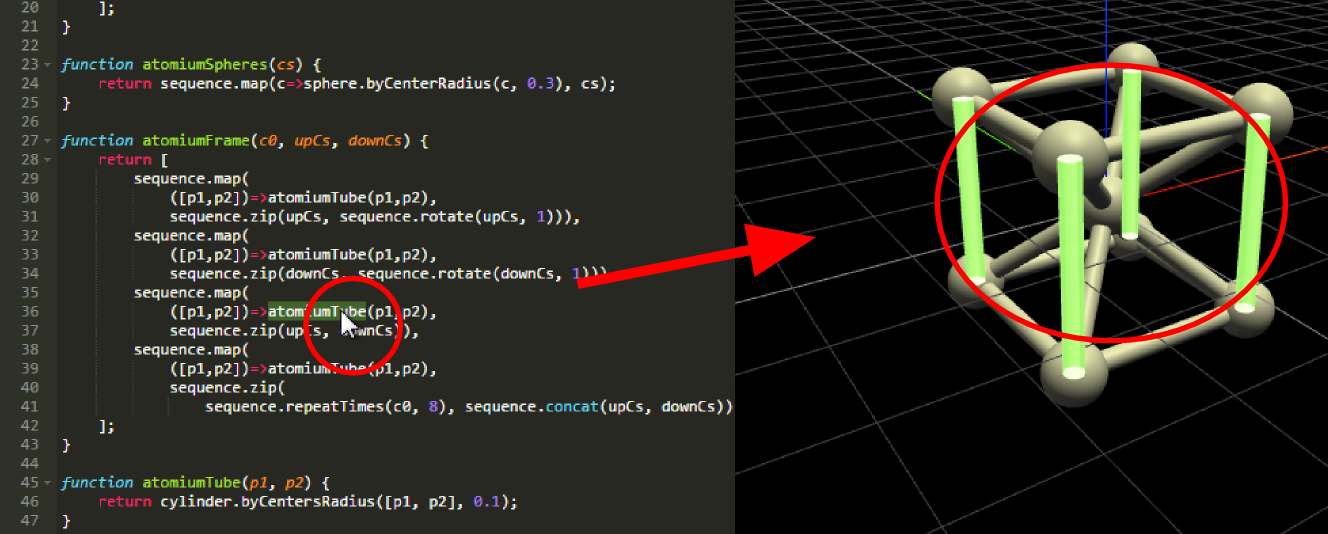
\includegraphics[width=1.0\textwidth]{./images/traceability_example/code_to_results_crop}
    \caption{From code to results.}
    \label{sub:code:to:results}
  \end{subfigure}

  \begin{subfigure}[b]{1.0\textwidth}
    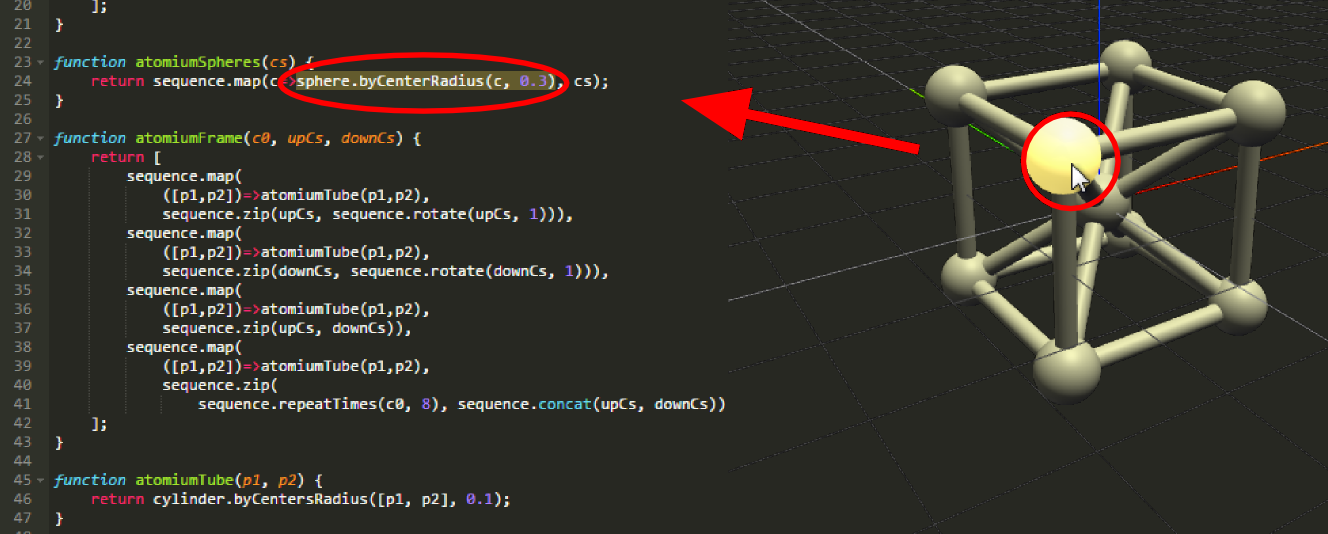
\includegraphics[width=1.0\textwidth]{./images/traceability_example/results_to_code_crop}
    \caption{From results to code.}
    \label{sub:results:to:code}
  \end{subfigure}
  \caption{Two examples of the traceability mechanism. The first from program to results and the second from results to program.}
  \label{fig:trace:example}
\end{figure}


\subsection{Running Programs}
\label{sec:run:progs}
One of the fundamental parts of the programming environment is that it runs programs.
To run programs, the environment needs to know which programming language is being used and to implement primitive operations the program has access to.
After knowing these, the environment must have a process to run the program and collect results to display them later.


\subsubsection{Programming Language}
Everyone can write a text or draw a diagram of what they want the computer to do.
However, if they do not use a concrete and unambiguous language that can be translated automatically by the computer, it will not be possible to get the computer to do what they want.

The environment has to use a programming language that fits the architect's needs.
It can either be an existing language with slight adaptations or a new one specially tailored for their needs.

Still, creating a new programming language is not realistic since it would require a great implementation effort to get a working version.
Moreover, since we want programs to run as fast as possible to be able to give architects immediate feedback, further effort would be needed to make it perform fast.

Furthermore, existing programming languages have had time to gather communities that can help the architect when he does not know how to do something or when he is having trouble correcting a bug.
A new programming language would have a severely limited community.
This suggests that we should use a programming language that already exists.

Architects' experience with programming can vary, however, we can assume that there are more novices than experts.
Like so, the environment needs to have a programming language is easy to learn and use.
We can consider programming languages that are commonly regarded as good introductory languages such as Python, Racket, and Processing as possible candidates.
Additionally, we can also consider DesignScript, since it was made specifically with design programming in mind, and also JavaScript, since it is readily available in web browsers and was originally made for web designers.

Programming languages have to be translated into the host's language.
For example, to run programs on a typical computer processor, they need to be translated into the {\tt x86} instruction set; to run programs on a virtual machine like the JVM, they need to be translated to its bytecode.
The same is true to run programs on a web browser.
In their case, instead of translating programs into an instruction set or a bytecode, they need to be translated into JavaScript.
Using JavaScript as the environment's language would spare us from a translation step as it is already the target language.
This lead us to choose JavaScript as the programming language supported by the environment.

After having a programming language, there still needs to be a concrete \gls{api} that supports the creation of \gls{gd} programs.
There are things that are essential to support, like the creation of geometry such as coordinates, lines, surfaces and solids.
Without the \gls{api} supporting it, the architect would need to implement these concepts even before tackling his design problem.
Furthermore, there are things that must not be done, like having side-effects.
If the \gls{api} includes operations that produce side-effects apart from creating new values, such as mutating arguments or changing global variables, the architect will have a harder time reasoning about the outcomes of programs.
These two things are essential to having a \gls{api} that supports \gls{gd}.
The \gls{api} provided by the environment adheres to these restrictions.

Still tied to the programming language and the \gls{api} provided to programs is how the environment gets the results from programs in order to be able to display them to the architect.

\paragraph{Alternatives for getting results}
We considered various alternatives for collecting the results of programs.
They are described in the following list:
\begin{itemize}
  \item {\bf Special entry point} Like in OpenJSCAD, we could require that every program must define a function with a special name (e.g. ``main'').
  The environment would then call this function and use its return value as the results of the program.

  \item {\bf Display function} Another way to get results from a program would be giving it access to an output function to the program.
  During its execution, the program would call this function, maybe several times, to produce its output.

  \item {\bf Imperative primitives} A third way to get results would be to add a side-effect to all the 3D object producing functions/primitives.
  Apart from creating the object, they would also add it to the program's results.
  This would be similar to having a display function, as all primitives become specialized display functions.

  \item {\bf Top-level expressions} A fourth way to get results would be to collect them from the expressions at top-level position within the program.
\end{itemize}

Each of this alternatives encourages a slightly different programming approach.
The {\it Imperative primitives} and {\it Display function} alternatives encourage an imperative programming approach, since the programmer must give instructions to create objects or display them.
The {\it Special entry point} and {\it Top-level expressions} alternatives, on the other hand, encourage a functional programming approach since the programmer must specify what objects constitute the results.

We wanted the environment to encourage users to follow a functional programming approach.
Therefore, we did not allow primitives to have side-effects and, like so, we have excluded the alternatives to get results that encouraged imperative programming, namely, {\it Imperative primitives} and {\it Display function}.

Having a {\it Special entry point} is similar to collecting the results of {\it Top-level expressions}, however, it requires the programmer to define a function that returns the results of the program.
When the programmer wants his program to have several results, he will have to aggregate them into a value to provide it as a return value.
This fact lead us to exclude using a {\it Special entry point} as the way the environment uses to collect results.

With all this in mind, we chose to collect the results of {\it Top-level expressions} as the way to collect program results.
Like this, it is easy for the programmer to specify the results of programs since he only has to write the expression at the program's top-level.
Moreover, this approach still encourages him to follow a functional programming approach.
Finally, Listing~\ref{lst:program:example} gives an example of what a program looks like in our environment.

\begin{listing}
\begin{minted}[linenos,frame=lines]{js}
const xyz = point.byXYZ;

function abacus(height, side) {
  return box.byBottomWidthHeightZ(xyz(0,0,0), [side, side], height);
}

function echinus(height, side, neckSide) {
  return coneFrustum.byBottomTopRadiusesHeight(xyz(0,0,0), neckSide/2, side/2, height);
}

function shaft(height, side, neckSide) {
  return coneFrustum.byBottomTopRadiusesHeight(xyz(0,0,0), side/2, neckSide/2, height);
}

function column(height, side, neckSide) {
  return [
    translate(abacus(height*0.05, side)).byZ(height*0.95),
    translate(echinus(height*0.05, side, neckSide)).byZ(height*0.90),
    shaft(height*0.90, side, neckSide)
  ];
}

column(6.00, 0.8, 0.7);
\end{minted}
\caption{An example of a program written our environment.}
\label{lst:program:example}
\end{listing}


%\subsubsection{Providing primitives / Runtime library / Primitive Library}
%\label{sub:provide:predefs}
%{\bf(what is the purpose of this subsubsection? I already talk about providing primitives in the next subsubsection...)}\\
%Any program needs to based upon functionality already provided by its host environment.
%It is this functionality that enables the program to produce results.
%
%But how does our solution do this for programs written by architects?
%We do this by defining all predefined functionality in a JavaScript module and then providing it to the function that represents the program as a parameter.
%Afterwards, we also add some code to the beginning of the program that will declare each primitive and extract the corresponding functionality from that parameter.


\subsubsection{Running process}
When the environment runs a program, it needs to do two things: (1) collect the results of the program; and (2) collect traceability data.
It does these two by instrumenting the program with additional calls to special functions that record the desired information, then running the program, and afterwards collecting the results from the instrumentation.
As stated in \ref{sec:traceability}, the collection of traceability data is optional since it adds a significant overhead to program execution, which may be undesired when programs start to take too much time to run.

To be able to perform the instrumentation, the environment parses the program using Esprima, a JavaScript parser,\footnote{\url{https://github.com/jquery/esprima} (last accessed on 10/10/2016)} to get its \gls{ast}.%
\footnote{The \gls{ast} conforms to a community standard. It can be found at \url{https://github.com/estree/estree} (last accessed on 10/10/2016).}

Afterwards, the \gls{ast} is transformed by: (1) adding a recording call to all top-level expression statements; and (2) adding a recording call to all function call expressions.
Figure~\ref{fig:instrument:example} exemplifies the transformation.
To let the recording functions know what top-level expression or function call is producing a result, we also provide them with identifiers for those expressions.

After this step, the environment creates a new function with the instrumented program as its body.
The primitives and recording functions are provided as parameters to this new function.

Finally, the newly created function is called and, afterwards, the recorded information is made available to the rest of the system.

\begin{figure}
  \centering
\begin{minipage}[t]{0.45\linewidth}
  \center{Before}
  \begin{minted}[frame=lines]{js}
let s = sphere.byRadius(5);
s;
  \end{minted}
\end{minipage}
\hspace{0.05\linewidth}
\begin{minipage}[t]{0.45\linewidth}
  \center{After}
  \begin{minted}[frame=lines]{js}
let s = recordCallResult(
   sphere.byRadius(5),
   /*function call ID*/);
recordTopLevelResult(
   s,
   /*top-level expression ID*/);
  \end{minted}
\end{minipage}
  \caption{A program before and after the transformation.}
  \label{fig:instrument:example}
\end{figure}


\subsubsection{Displaying Results}
After running the program, the environment needs to display a rendering of the results to the architect.
Displaying results is deeply tied to what programs can produce since their results must be converted to a representation that can be rendered.
The \gls{api} used by those programs is what determines which results can be produced.
The environment uses THREE.js for 3D rendering.
By using THREE.js, the implementation effort is reduced since, on top of implementing rendering, THREE.js also implements several geometric primitives useful for GD and implements ray-casting.
However, since the environment provides a functional \gls{api} and THREE.js's API is imperative, it needs to cover the differences between these two \glspl{api}.

The main difference between them lies in how they support reuse.
THREE.js's \gls{api} makes it difficult to reuse objects since it only allows scenegraph objects to have one parent.
If the programmer wants to reuse one object, he has to clone it.
The environment's \gls{api}, on the other hand, does not impose this rule.
To cover the difference, we use two steps:
(1) we run the program using the functional \gls{api}, creating intermediary results;
and (2) we convert those results to objects from THREE.js's \gls{api}, cloning them when necessary.
Figure~\ref{fig:display:results} shows the overall process from having a program to displaying its results, while Figure~\ref{fig:results:vs:three} shows an example of the transformation that occurs between intermediary results and THREE.js objects.

After having results converted to THREE.js objects, the environment issues their rendering repeatably as the architect interacts with the 3D view.

The environment also keeps record of the correspondence between intermediary results and THREE.js objects.
Together with the correspondence between program nodes and intermediary results, this information is used to enable support for showing traceability.

\begin{figure}
  \centering
  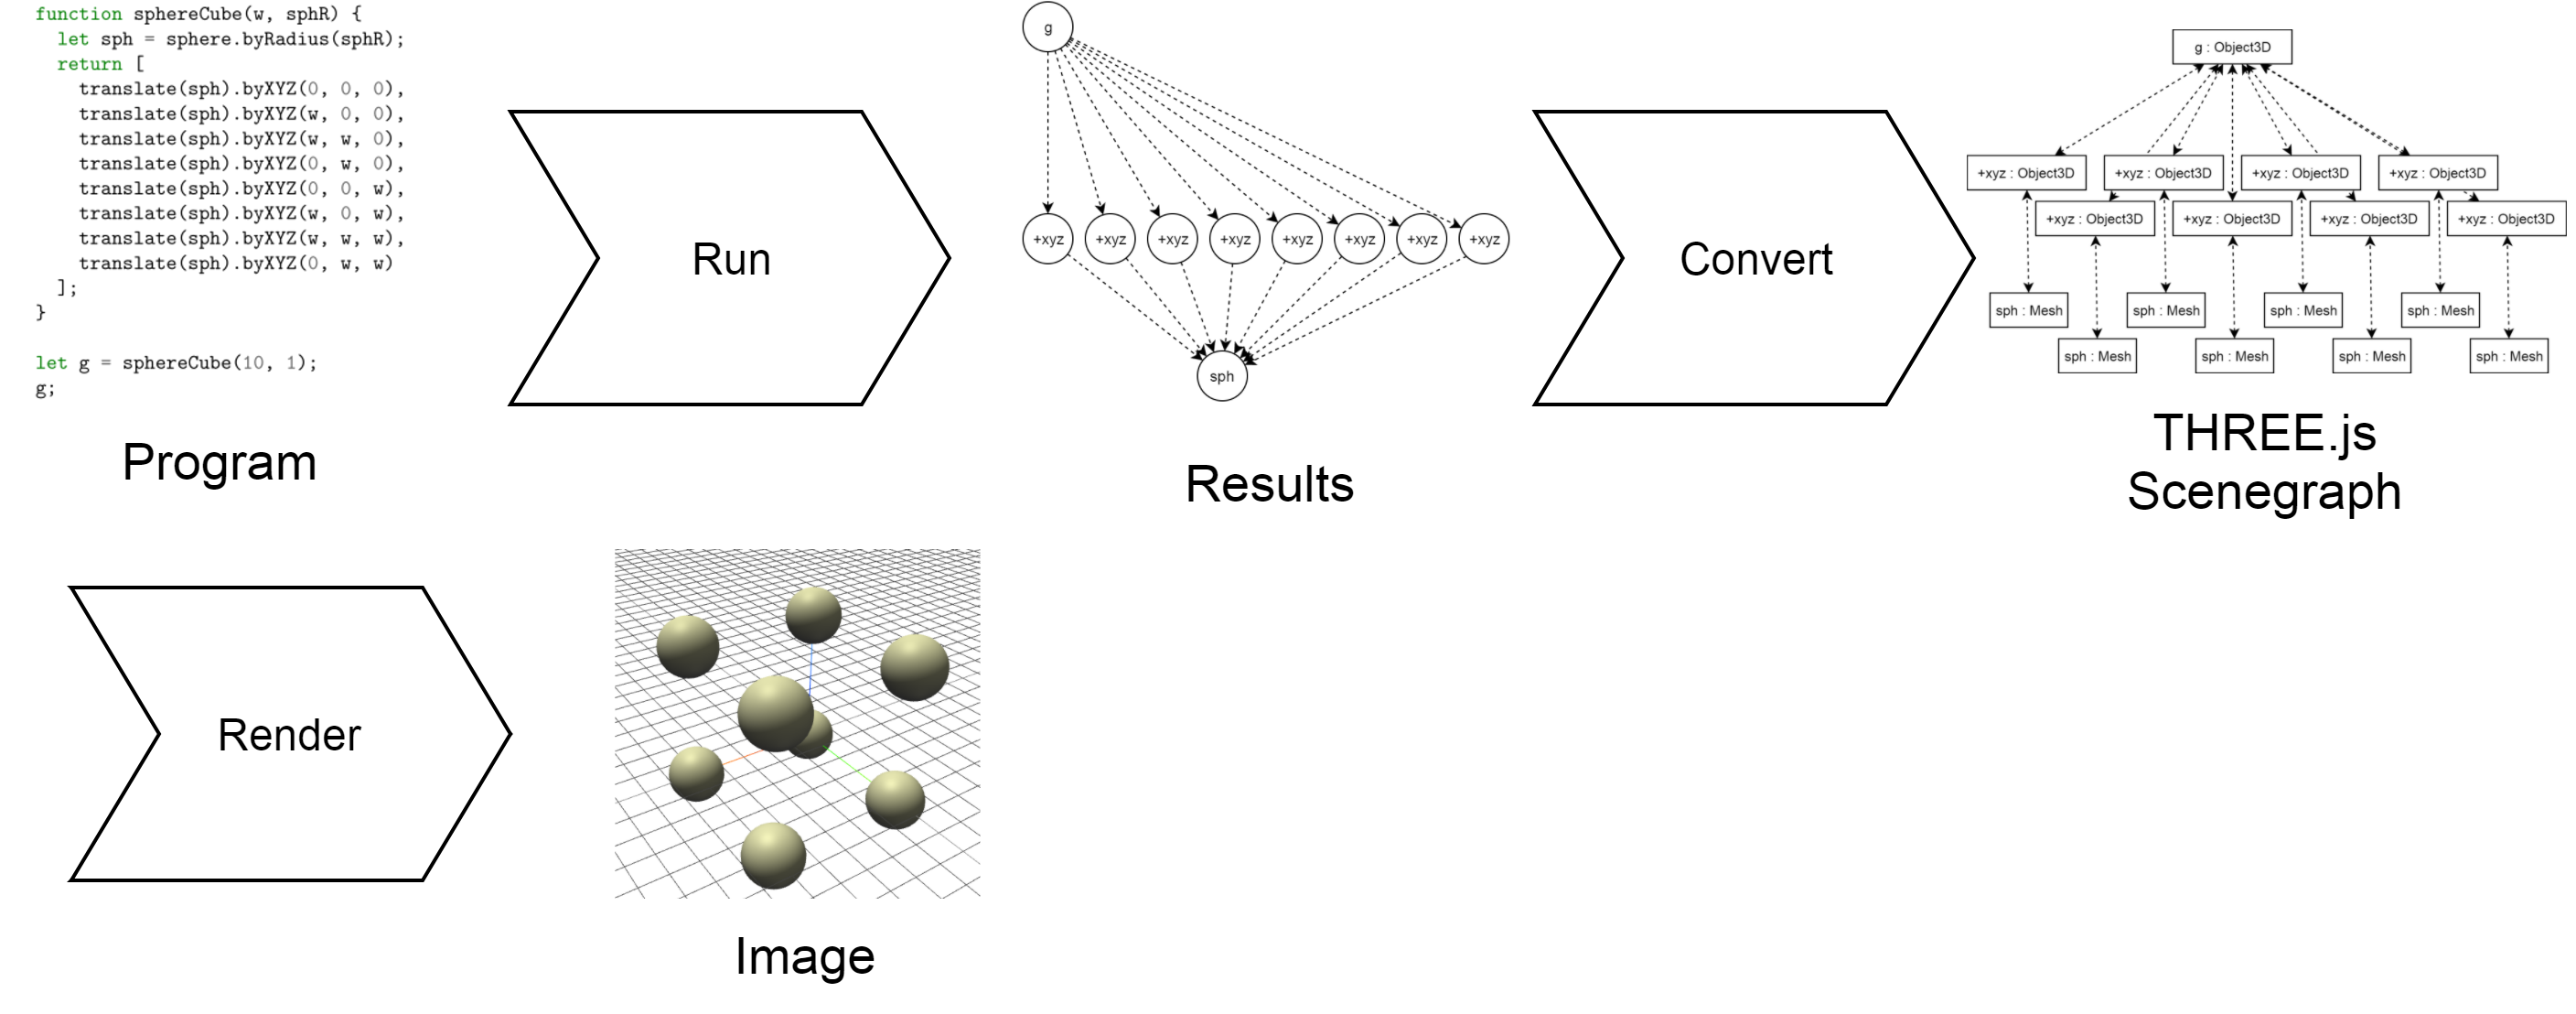
\includegraphics[width=1.0\textwidth]{./images/display_results/display_results}
  \caption{The process used to display results.}
  \label{fig:display:results}
\end{figure}

\begin{figure}
  \centering
  \begin{subfigure}[b]{0.45\textwidth}
    \includegraphics[width=1.0\textwidth]{./images/display_results/results}
    \caption{Program results}
  \end{subfigure}
  \begin{subfigure}[b]{0.45\textwidth}
    \includegraphics[width=1.0\textwidth]{./images/display_results/three}
    \caption{THREE scenegraph}
  \end{subfigure}
  \caption{Comparison of program results structure and THREE.js scenegraph.}
  \label{fig:results:vs:three}
\end{figure}


\section{Remote CAD Service / Exporting to CAD}
The last task that the environment needs to support is exporting to \gls{cad} applications.

As opposed to the other tasks, exporting to a \gls{cad} application requires the environment to communicate with other appications.
To do so, the environment must locate the \gls{cad} application and connect to it.
In addition, there must be a well-defined interface of operations that can be performed in the \gls{cad}, which need to cover the operations that can be performed in the web page, as well as operations for managing the \gls{cad}'s document.

To make communication possible, we have implemented an application that the architect must install and run in his computer.
This application serves as a bridge between \gls{cad} applications installed in the computer and the environment running in the web page.
After being started, the application detects which \glspl{cad} are installed in the computer and connects to the ``environment directory'' so it can be discovered by the web page.
When the architect needs to export a program to his \gls{cad} application, the web page connects to the application in his computer through the ``environment directory'' and starts to send requests to it, in order to create shapes in the \gls{cad} application.
The architecture for this part of the solution is illustrated in Figure~\ref{fig:remote:cad:archi}.
As long as these components can communicate with each other, the system can work.
In the extreme, each can be running in a distinct computer, as long as all computers are connected to the same network.

Figure~\ref{fig:remote:cad:example} shows an example of the export to \gls{cad} functionality in action.
The architect has created a program using the web page environment.
After selecting AutoCAD and SketchUp as export destinations, he starts the export process and, some time later, the model resulting from running the program is available in both \gls{cad} applications.

Note that it is only needed to install the application when the architect is finally ready to get the program's results on a \gls{cad} application.
Furthermore, the application only needs to be installed in the computer that actually has the \gls{cad} application installed, while the rest only accesses the web page.


\subsection{Implementation}
We implemented the remote CAD application as a small Racket server.
It expects to receive HTTP requests for operations like adding shapes to the currently selected \gls{cad} applications or deleting all shapes they may have.
It also expects requests for specifying what \gls{cad} applications are selected.
%{\bf(appendix has remote CAD service API?)}

Apart from the connection between the remote CAD application and the web page, there also needs to be a connection between the remote CAD application and the \gls{cad} applications.
Different \glspl{cad} have different \glspl{api} so the application needs to know how to interact with each one.

Instead of implementing the connection with \gls{cad} applications itself, the application uses Rosetta as an intermediate.
This way, it only has to cover the semantic differences between Rosetta's \gls{api} and the remote CAD service's \gls{api}.

In reality, when the architect wants to export to \gls{cad}, it is likely that he is using the web environment in the same computer where he has the \gls{cad} application installed.
Like so, the web page, the remote CAD application and the \gls{cad} applications run in the same computer.
With this in mind, we chose to temporarily host the web page containing the \gls{ide} in the remote CAD application's server.
Using this setup, it is easier to test the communication between the page and the application.
This setup also avoids dealing with cross-origin restrictions imposed by web browsers for \gls{ajax} requests.

\begin{figure}
  \centering
  \includegraphics[width=1.0\textwidth]{./images/export_archi_over/export_archi_over}
  \caption{Illustration of the remote CAD service's architecture.}
  \label{fig:remote:cad:archi}
\end{figure}


\begin{figure}
  \centering
  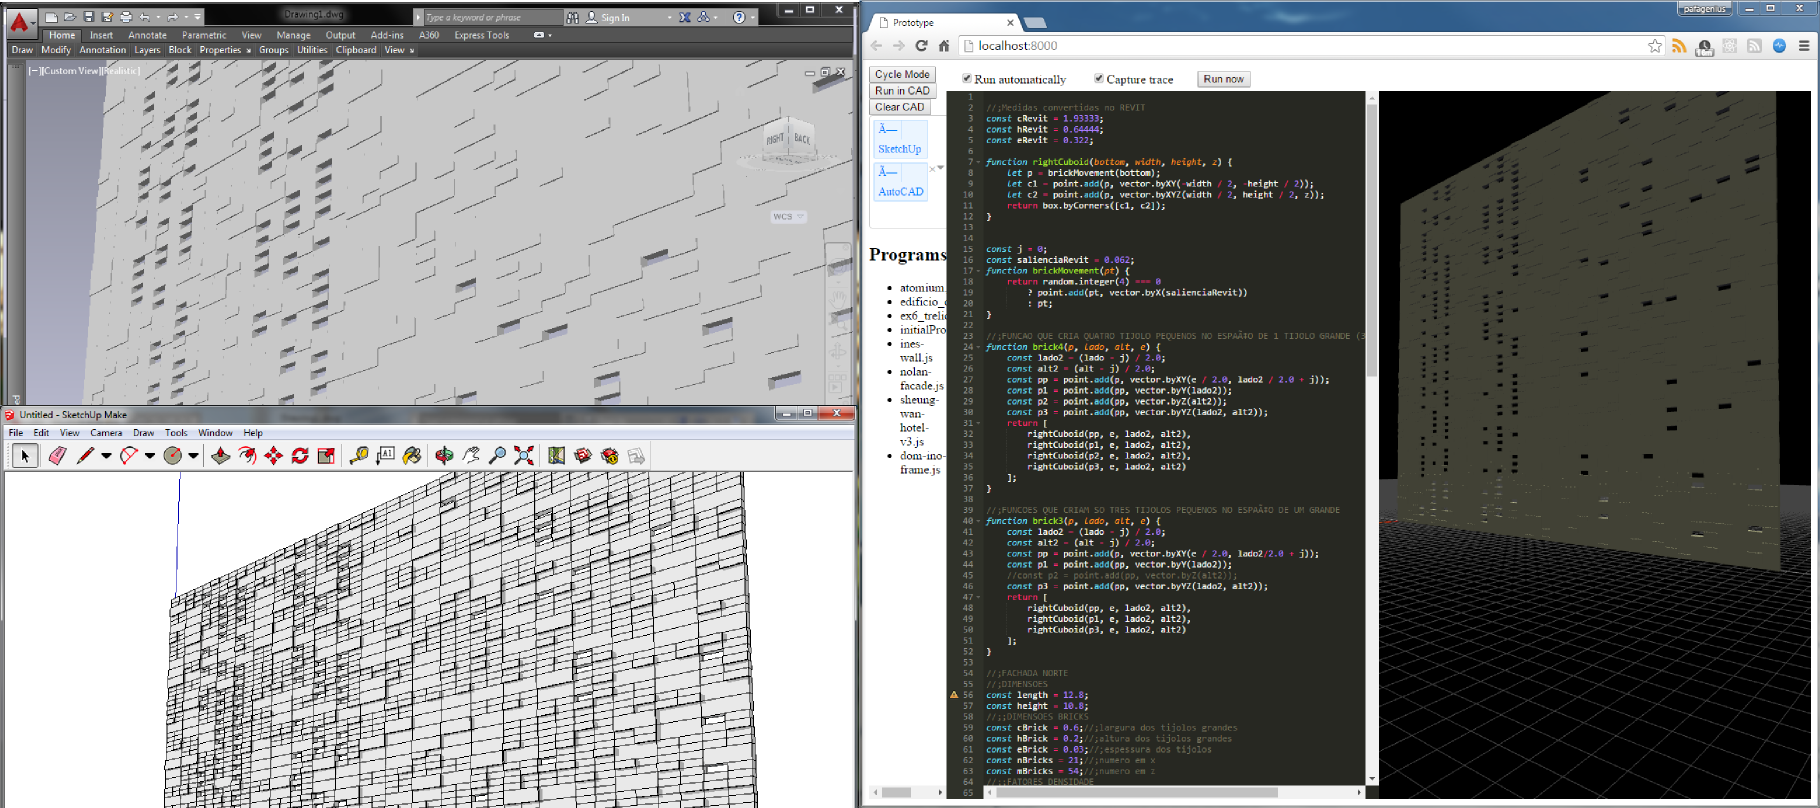
\includegraphics[width=1.0\textwidth]{./images/remote_cad_example/remote_cad_example}
  \caption[An example of the remote CAD service.]{An example of the remote CAD service. The results of the program have been passed to both AutoCAD and SketchUp.}
  \label{fig:remote:cad:example}
\end{figure}


%Design principles / Guiding ideas
%- Ideas based on observations from related work?

%Architecture - Show the overview of the architecture
%- Web page + remote CAD service

%Web page
%- Architecture
%- Page Layout
%- Features / What needs to be done by the IDE?
%   - Discussion + Decision
%   - Implementation
%- Problems
%   - Adjusting source code values
%   - Instrumenting and running programs
%     - Getting results / What is a program?
%     - Providing primitives/predefined bindings
%     - Handling traceability
%   - (Running programs blocks the UI)
%   - Displaying 3D results

%Remote CAD service
%- Architecture
%- Problems
%   - Supporting multiple CADs
%   - Defining the API

%Problem: Handling CAD communication
